\documentclass[10pt]{article}

\usepackage[T2A]{fontenc}
\usepackage[utf8]{inputenc}
\usepackage[english, russian]{babel}
\usepackage{amssymb}
\usepackage{url}

\usepackage{fancyvrb}
\usepackage{color}
\usepackage{pdfpages}
\usepackage{caption}
\usepackage{subcaption}

\usepackage{listings}
\usepackage{algpseudocode}
\usepackage{algorithmicx}

\usepackage{cmap}
\usepackage{natbib}
\setlength{\bibsep}{0.2pt}

\newtheorem{definition}{Определение}

\algnewcommand\algorithmicswitch{\textbf{switch}}
\algnewcommand\algorithmiccase{\textbf{case}}
\algnewcommand\algorithmicassert{\texttt{assert}}
\algnewcommand\Assert[1]{\State \algorithmicassert(#1)}

\algdef{SE}[SWITCH]{Switch}{EndSwitch}[1]{\algorithmicswitch\ #1\ \algorithmicdo}{\algorithmicend\ \algorithmicswitch}
\algdef{SE}[CASE]{Case}{EndCase}[1]{\algorithmiccase\ #1}{\algorithmicend\ \algorithmiccase}

\algtext*{EndSwitch}
\algtext*{EndCase}
\algtext*{EndWhile}
\algtext*{EndIf}
\algtext*{EndFor}
\algtext*{EndFunction}
\algtext*{EndProcedure}

\title{Динамически формируемый код: синтаксический анализ \\ контекстно-свободной аппроксимации}
\author{
    Дмитрий Ковалев, Семён Григорьев \\
    \textit{Санкт-Петербургский государственный университет,} \\
    \textit{Россия, 199034, Санкт-Петербург, Университетская наб. 7/9} \\
    \url{dmitry.kovalev-m@ya.ru}, \url{semen.grigorev@jetbrains.com} }
\date{}

\begin{document}

\maketitle

\begin{abstract}
Многие программы в процессе работы формируют из строк исходный код на некотором языке программирования и передают его для исполнения в соответствующее окружение (пример --- dynamic SQL). 
Для статической проверки корректности динамически формируемого выражения используются различные методы, одним из которых является синтаксический анализ регулярной аппроксимации множества значений такого выражения. 
Аппроксимация может содержать строки, не принадлежащие исходному множеству значений, в том числе синтаксически некорректные. 
Анализатор в данном случае сообщит об ошибках, которые на самом деле отсутствуют в выражении, генерируемом программой. 
В данной статье будет описан алгоритм синтаксического анализа более точной, чем регулярная, контекстно-свободной аппроксимации динамически формируемого выражения.
\\
\\
\textbf{Ключевые слова:} синтаксический анализ, динамически формируемый код, контекстно-свободные грамматики, GLL, GFG, dynamic SQL, DSQL 
\end{abstract}

\section*{Введение}
Современные языки программирования общего назначения поддерживают возможность работы со строковыми литералами, позволяя формировать из них выражения при помощи строковых операций. 
Строковые выражения могут создаваться динамически, с использованием таких конструкций языка, как циклы и условные операторы. 
Данный подход широко используется, например, при формировании SQL-запросов к базам данных из программ, написанных на Java, C$\#$ и других высокоуровневых языках (листинг \ref{lst:example}).

\begin{figure}[h]	
	\vspace{-10pt}
	\lstset{language=[Sharp]C,
		showstringspaces=false,
		basicstyle=\small,
		keywordstyle=\bfseries,,	
	}
	\begin{lstlisting}[caption={Динамически формируемый SQL-запрос}, label={lst:example}, captionpos=b]
private void Example (bool cond) {
    string columnName = cond ? "name" : "address";
    string queryString = 
        "SELECT id, " + columnName + " FROM users";
    Program.ExecuteImmediate(queryString);
}
	\end{lstlisting}
	\vspace{-10pt}
\end{figure}

Недостаток такого метода генерации кода заключается в том, что формируемые выражения, с точки зрения компилятора, являются обычными строками и не проходят статические проверки на корректность и безопасность, что приводит к ошибкам времени исполнения и усложняет разработку и сопровождение системы. 
Включение обработки динамически формируемых строковых выражений в фазу статического анализа осложняется тем, что такие выражения, в общем случае, невозможно представить в виде линейного потока, который принимают на вход традиционные алгоритмы лекcического/синтаксического анализа. 

Для решения данной проблемы были разработаны различные методы статического анализа множества значений формируемого выражения. 
Как правило, язык, на котором написана исходная программа, тьюринг-полон, что делает невозможным проведение точного анализа. Поэтому распространенным подходом является построение некоторой аппроксимации рассматриваемого множества. 
Ряд предложенных ранее решений использует для анализа \textit{регулярную аппроксимацию} --- множество строк, генерируемых программой, аппроксимируется сверху регулярным языком, и анализатор работает с его компактным представлением, таким как регулярное выражение или конечный автомат.

В магистерской диссертации \cite{gll_reg} был описан алгоритм, позволяющий проводить синтаксический анализ регулярной аппроксимации (конечного автомата, представленного в виде графа) множества значений динамически формируемого выражения. Основой для данного алгоритма служит алгоритм обобщенного синтаксического анализа Generalized LL (GLL, \cite{gll}).
Такой подход позволяет получать конечное представление леса разбора \cite{sppf} корректных строк, содержащихся в аппроксимации множества значений выражения. Это представление может быть использовано для проведения более сложных видов статического анализа и для целей реинжиниринга.

В данной статье будет представлен алгоритм синтаксического анализа, который основан на описанной выше модификации GLL, но работает с более точной, чем регулярная, контекстно-свободной аппроксимацией множества значений динамически формируемого выражения. 
Использование более точной аппроксимации позволяет снизить количество ложных синтаксических ошибок, возникающих в результате того, что аппроксимирующее множество может содержать строки, осутствующие среди значений искомого выражения.
\section{Обзор}

Под \textit{контекстно-свободной аппроксимацией} подразумевается грамматика, описывающая контекстно-свободный язык, который содержит в качестве подмножества возможные значения динамически формируемого выражения. 
Идея использования такой аппроксимации была заимствована из существующих работ в области анализа динамически формируемого кода, краткий обзор которых будет приведен в данной секции. 
Алгоритм синтаксического анализа регулярной аппроксимации на основе GLL был адаптирован нами для работы c графовым представлением КС-грамматик. 
В качестве такого представления мы использовали Grammar Flow Graph (GFG,~\cite{gfg}). Описания оригинального алгоритма и GFG также включены в обзор. 

\subsection{Подходы к анализу динамически формируемых выражений}

Существует два основных подхода, позволяющих проводить различные виды анализа динамически формируемого кода. 
Один из них основан на проверке включения языка, аппроксимирующего множество значений динамически формируемого выражения, в эталонный контекстно-свободный язык, заданный пользователем. 
Данный подход был реализован в инструментах Java String Analyzer (JSA,~\cite{jsa}) и PHP String Analyzer (PHPSA,~\cite{phpsa}).
Получение аппроксимации в них реализовано следующим образом --- из исходного кода программы извлекается набор dataflow-уравнений, описывающих значения строковых переменных, которые участвуют в генерации выражения. 
Эти уравнения затем интерпретируются как контекстно-свободная грамматика, описывающая аппроксимирующий язык. 
PHPSA работает непосредственно с такой грамматикой, используя эвристики (т.к. в общем случае задача о включении КС-языков неразрешима~\cite{lang_inclusion}); в JSA контекстно-свободный язык дополнительно аппроксимируется регулярным.

Другой подход заключается в проведении синтаксического анализа аппроксимации множества значений выражения. 
Такое решение позволяет не просто ответить на вопрос о включении языков, но и реализовать дополнительную функциональность, такую как вычисление семантики или рефакторинг. 
К методам, основанным на данном подходе, можно отнести алгоритмы синтаксического анализа регулярной аппроксимации на базе семейства GLR~\cite{alvor, rnglr_reg} и GLL-алгоритмов~\cite{gll_reg}, а также алгоритм абстрактного синтаксического анализа~\cite{a_lr}, позволяющий совместить синтаксический анализ с решением dataflow-уравнений, получаемых при помощи PHPSA.

\subsection{Синтаксический анализ регулярной аппроксимации на основе GLL}

Generalized LL (GLL)~\cite{gll} --- алгоритм синтаксического анализа, позволяющий, в отличие от классических LL-анализаторов, работать с произвольными контекстно-свободными грамматиками. 
При этом, GLL сохраняет такие важные свойства алгоритмов нисходящего разбора, как интуитивная связь с грамматикой и простота отладки и диагностики ошибок.

Основной идеей GLL является использование дескрипторов, позволяющих полностью описывать состояние анализатора в текущий момент времени.

\begin{definition}
    Дескриптор --- это четверка (L, u, i, N), где
    \begin{itemize}
        \setlength\itemsep{0em}
        \item L --- текущая позиция в грамматике вида $A \rightarrow \alpha \cdot \beta$
        \item u --- текущая вершина Graph Structured Stack (GSS,~\cite{tomita})
        \item i --- позиция во входном потоке
        \item N --- построенный на данный момент узел дерева вывода  
    \end{itemize}
\end{definition}  

В процессе работы поддерживается глобальная очередь дескрипторов. В начале каждого шага исполнения алгоритм берет следующий в очереди дескриптор и производит действия в зависимости от позиции в грамматике и текущего входного символа. 
Для обработки неоднозначностей в грамматике алгоритм добавляет дескрипторы для каждого возможного пути анализа в конец очереди. Результат работы алгоритма --- множество деревьев разбора строки (лес разбора) --- представляется в виде Shared Packed Parse Forest (SPPF)~\cite{sppf}.

В рамках магистерской диссертации~\cite{gll_reg} на базе GLL был разработан алгоритм для синтаксического анализа регулярной аппроксимации множества значений динамически формируемого выражения. 
Под регулярной аппроксимацией здесь понимается детерминированный конечный автомат над алфавитом токенов (рис.~\ref{fig:app_r}). Оригинальный GLL-алгоритм был модифицирован для работы с нелинейным входом. 
Дескрипторы нового алгоритма хранят номер вершины входного графа вместо позиции в линейном потоке. Также, на шаге исполнения просматривается не единственный входной символ, а все ребра, исходящие из текущей вершины. Псевдокод данного алгоритма можно увидеть в приложении \ref{gll_code}. Основная логика работы представлена в функциях \textbf{dispatcher} (извлечение дескрипторов из очереди) и \textbf{processing} (анализ исходящих из текущей вершины ребер).

\subsection{Grammar Flow Graph}

Grammar Flow Graph (GFG,~\cite{gfg}) --- связный помеченный граф, узлы которого соответствуют позициям в грамматике ($A \rightarrow \alpha \cdot \beta$). Различают следующие типы узлов ($X$ --- нетерминальный символ, $t$ --- терминальный):
\begin{itemize}
    \setlength\itemsep{-0.2em}
    \item[--] $A \rightarrow \alpha \cdot X \beta   $ --- call
    \item[--] $A \rightarrow \alpha X \cdot \beta$ --- return
    \item[--] $A \rightarrow \cdot \alpha$ --- entry
    \item[--] $A \rightarrow \alpha \cdot$ --- exit
    \item[--] $A \rightarrow \alpha \cdot t \beta$ --- scan
\end{itemize}
Для обозначения подграфа, представляющего продукции, имеющие в левой части нетерминал $A$, дополнительно используются узлы с метками $.A$ (start-узел) и $A.$ (end-узел). Подробное описание GFG можно найти в оригинальной статье.

Приведем определение выводимости строки в грамматике в терминах GFG. Для этого нам потребуется также определить понятие сбалансированного пути.

\begin{definition}
    Сбалансированным путем в GFG называется путь, подпоследовательность call- и return-узлов которого сбалансирована. 
\end{definition}

\begin{definition}
    Строка $w$ выводима в грамматике, если в GFG существует сбалансированный путь из узла $.S$ в узел $S.$ (здесь S --- стартовый нетерминал грамматики), и $w$ может быть получена конкатенацией меток на ребрах, содержащихся в данном пути. 
\end{definition}

\begin{figure}[!h]
	\centering
	\begin{subfigure}[h!]{0.33\textwidth}
		\centering
		\begin{minipage}{5cm}
			\begin{Verbatim}[commandchars=\\\{\}]
expr = \textcolor{red}{"a"}
while (...)
  expr = \textcolor{red}{"("} + expr + \textcolor{red}{")"}
print expr
			\end{Verbatim}
		\end{minipage}
		\caption{Исходный код}
		\label{fig:code}
	\end{subfigure}
	\hfill
	\begin{subfigure}[h!]{0.3\textwidth}
		\centering
		$
		\begin{array}{crcl}
			&s' &::=& s \\
			&s & ::= & \mbox{\texttt{LBR }} s \mbox{\texttt{ RBR}}\\
			&s & ::= & \mbox{\texttt{A}}
		\end{array}
		$
		\caption{КС-аппроксимация}
		\label{fig:app_cf}
	\end{subfigure}
	\hfill
	\begin{subfigure}[h!]{0.3\textwidth}
		\centering
		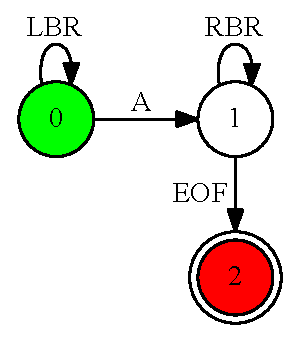
\includegraphics[width=2.5cm]{pictures/kovalev-spbu-reg_app}
		\caption{Регулярная}
		\label{fig:app_r}
	\end{subfigure}
	\caption{Исходный код и примеры аппроксимаций}
	\label{example}
\end{figure}

\begin{figure}[h]
    \centering
    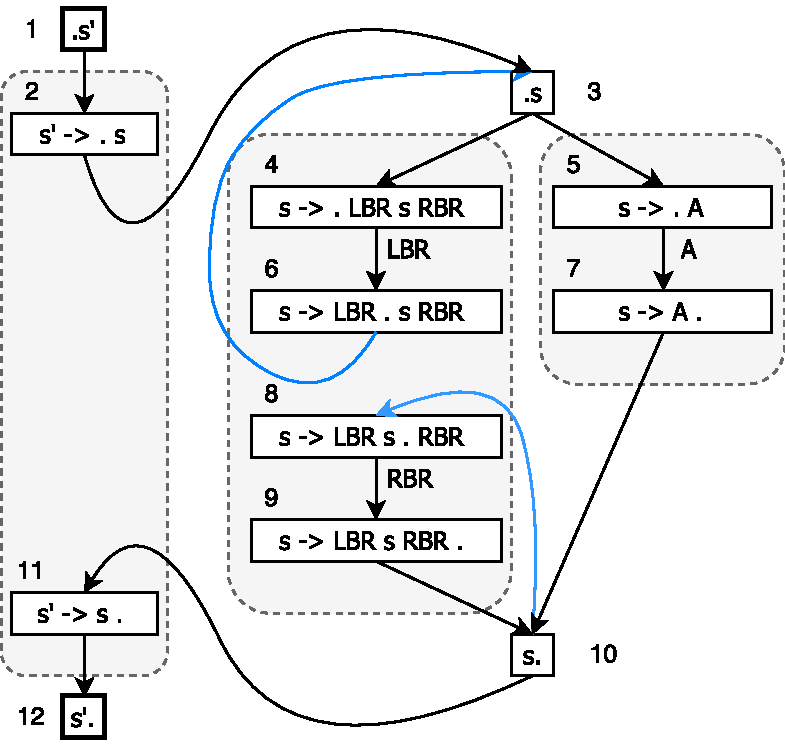
\includegraphics[width=0.5\textwidth]{pictures/kovalev-spbu-gfg_enum}
    \caption{GFG для грамматики \ref{fig:app_cf}}
    \label{fig:gfg}
\end{figure}

\section{Синтаксический анализ контекстно-свободной аппроксимации}

Наш алгоритм принимает на вход управляющие таблицы LL-анализа, построенные по эталонной грамматике, и GFG, который является представлением КС-грамматики --- аппроксимации множества значений выражения. 
Мы переиспользуем основные структуры данных и функции описанного ранее алгоритма анализа регулярной аппроксимации на основе GLL, расширяя данный подход для корректной обработки GFG.

Алгоритм последовательно обходит узлы GFG, производя синтаксический анализ порождаемых им строк. 
Для правильного построения таких строк, согласно определению выводимости строки в GFG-грамматике, для каждого просматриваемого пути необходимо поддерживать баланс call- и return-узлов. 
То есть, при прохождении пути алгоритм должен манипулировать дополнительным стеком (назовем его \textit{CR-стеком}). 
При достижении call-узла в стек добавляется номер return-узла, соответствующего ему; при достижении end-узла необходимо снять со стека номер return-узла и продолжить обход из него. 

Для экономии памяти мы не храним CR-стек для каждой из текущих ветвей работы алгоритма (напомним, что GLL-алгоритм может одновременно рассматривать несколько вариантов разбора строки). 
Вместо этого множество CR-стеков, по аналогии с основным стеком GLL-анализатора, представляется в виде GSS. 
Пример можно увидеть на рисунке \ref{fig:gss}. GSS позволяет хранить только одну копию общих префиксов нескольких стеков, каждый путь в нем соответствует отдельному CR-стеку.

\begin{figure}[h]
	\centering
	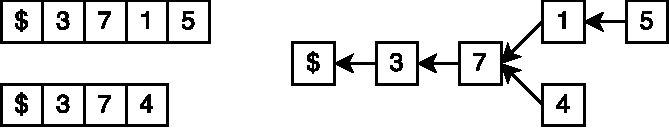
\includegraphics[width=6cm]{pictures/gss_cr}
	\caption{Структурированный в виде графа стек}
	\label{fig:gss}
\end{figure}

Для хранения указателя на текущую вершину стека мы добавили в дескрипторы дополнительное поле. 
Таким образом, дескриптором в нашем алгоритме называется пятерка вида $(L, u, i, N, s)$, где $i$ --- номер вершины GFG, $s$ --- указатель на вершину CR-стека в GSS, остальные поля аналогичны тем, которые представлены в дескрипторах оригинального GLL-алгоритма.

Другой особенностью работы с GFG является то, что он, в отличие от регулярной аппроксимации --- детерминированного конечного автомата, допускает возможность неоднозначного выбора пути обхода. 
Подобная ситуация возникает при наличии в исходной грамматике нескольких продукций, содержащих в левой части одинаковый нетерминал. 
Например, GFG на рисунке \ref{fig:gfg} содержит start-узел под номером 3, из которого выходит два ребра с пустой меткой (аналог $\epsilon$-переходов в конечном автомате).

Механизм дескрипторов позволяет решать проблему недетерминированного выбора пути --- для каждого из возможных вариантов создается отдельный дескриптор, который добавляется в очередь исполнения. 
Вернемся к примеру с узлом 3 на рисунке \ref{fig:gfg}. Пусть в текущий момент времени мы имеем дескриптор $(L_1, u_1, i_1, N_1, s_1)$. 
При рассмотрении ребер, выходящих из узла 3, будут созданы дескрипторы $(L_1, u_1, 4, N_1, s_1)$ и $(L_1, u_1, 5, N_1, s_1)$. Если ранее такие дескрипторы не создавались (для контроля за этим в GLL поддерживается глобальное множество создаваемых дескрипторов), они будут добавлены в очередь.

Функции \textbf{dispatcher} и \textbf{add} (проверка и добавление в очередь дескриптора) алгоритма анализа регулярной аппроксимации были незначительно изменены нами для работы с расширенными дескрипторами. 
Функция \textbf{processing} и методы для работы с основным стеком и построения SPPF переиспользованы без изменений.
Обработка start/call/exit-узлов и контроль за состоянием CR-стеков были реализованы во вспомогательной функции \textbf{closure}, псевдокод которой приведен ниже.
Она исполняется перед вызовами \textbf{dispatcher} и \textbf{processing}, производя рекурсивный обход GFG до тех пор, пока не встретит start- или scan-узел. 
При достижении start-узла создаются дескрипторы для каждого из возможных путей, и управление переходит к \textbf{dispatcher};
scan-узел обрабатывается функцией \textbf{processing} так же, как и вершина конечного автомата в оригинальном алгоритме.

\section{Closure properties of languages with polynomial rational indices}
\label{sec:closure}
Given a context-free language $L$ with a polynomial rational index, it is interesting to find which language operations preserve this property.  Boasson et al. \cite{RatBasic} give following useful relations for polynomial indices of two languages $L$ and $L'$.
\begin{theorem}[\cite{RatBasic}]
Context-free languages with polynomial rational indices are closed under intersection with a regular language, union, concatenation, homomorphism and inverse homomorphism. More precisely,
\begin{itemize}
\item $\rho_{L \cup L'} \le  \max{(\rho_L, \rho_{L'})} $
\item $\rho_{LL'} \le \rho_L + \rho_{L'}$
\item $\rho_{L \cap R}(n) \le \rho_L(nm)$, where $R$ is a regular language recognised by an $m$-state automaton
\item $\rho_{h(L)}(n) \le \rho_L(n)$ and $\rho_{h^{-1}(L)}(n) < n(\rho_L(n) +1)$, where $h: \Sigma^* \rightarrow \Delta^*$ is a homomorphism.
\end{itemize}
\end{theorem}
From the relations above it is easy to see that the family of context-free languages with polynomial rational indices is a full trio. Every full trio is closed under prefix and quotient with regular languages. Obviously, CFLs with polynomial rational indices languages are closed under reversal.  Next we show that context-free languages with polynomial rational indices are closed under Kleene star and insertion of a regular language (or context-free language with a polynomial rational index).
\begin{theorem}
Context-free languages with polynomial rational indices are closed under Kleene star and insertion of a regular language  (or context-free language with a polynomial rational index). Particularly,
\begin{itemize}
\item $\rho_{L^*}(n) \le n(\rho_L(n))$
\item $\rho_{LL'} \le \rho_L + \rho_{L'}$
\end{itemize}
\end{theorem}
\begin{proof}
\textit{Kleene star.} Let $G = (\Sigma, N, P, S)$ and $L(G)$ be a language with polynomial rational index. Consider language $L^{+}$, which grammar $G_1$ has the start nonterminal $S_1$. By definition of the Kleene plus operation, a rightmost derivation from $S_1$ generates a sequence of one or more start nonterminals $S$ from $G$, each of which generates some string in $L(G)$. Let $D$ be a directed labelled graph with $n$ nodes. Suppose there are nodes $u$ and $v$ in $D$ such that:
\begin{enumerate}
\item $v$ is not $L(G)$-reachable from $u$ and
\item $v$ is  $L^+$-reachable from $u$
\end{enumerate}
Then $v$ is reachable from $u$ via concatenation of words in $L(G)$. Consider the longest shortest path $u\pi_1 v$ between $u$ and $v$. It can be obtained by joining $(S, u, i), (S, i, j), ..., (S, w, v)$ into $(S_1, u, v)$.  If $L$ has the polynomial rational index, then for every realizable triple $(A, i, j)$ corresponding shortest path $i \pi j$ has at most polynomial length. There are no more than $O(n)$ such triples in concatenation because there are no repetitions of the same node in the sequence of start and end nodes of triples (otherwise $u\pi_1 v$ is not the shortest path, for example, path $u \rightarrow i \rightarrow k \rightarrow l \rightarrow i \rightarrow j \rightarrow v$ can be replaced with shorter path $u \rightarrow i  \rightarrow j \rightarrow v$), so $u\pi_1 v$ has at most polynomial length. In other words, we have $\rho_{L^+}(n) \le n(\rho_L(n))$.
\\
Family of languages with polynomial rational indices is a full trio closed under union, concatenation and Kleene star, therefore it is a full ALF. Full AFLs is known to be closed under substitution.
\\
\textit{Insertion of a regular language.} To prove closure under insertion of a regular language, the following PDA can be constructed. Let $L$ be a context-free language with polynomial rational index and let $M$ be a PDA recognizing $L$. New PDA $M'$ for insertion of a regular language $R$ recognized by finite automation $F$ into $L$ can be obtained as follows: duplicate all states in $M$, initial state is placed in first set and final states reside in the second set. Every state in the first set has its own copy of outgoing arcs of the initial state of $F$. Every ingoing arc of final state of $F$ is connected directly to every state of the second set of $M$. In other words, every state from the first set is the initial state of $F$ and every state from the second set is a final state of $F$. All arcs from $F$ are labelled the same way as they are labelled in $F$.
Consider intersection of $M'$ and arbitrary finite automotion $F'$ with $n$ states. The longest non-empty shortest path $i \pi j$ in the intersection of $M'$ and $F'$ consists of three sub-paths: $i\pi_1k$, $k\pi_2m$ and $m\pi_3j$, where $i\pi_1k$ ($m\pi_3j$) is the shortest paths in the intersection of $F'$ and first (second) set of states of $M$ respectively, and $k\pi_2m$ is the shortest path in the intersection of $F'$ and $F$. $k\pi_2m$ has at most polynomial length because all regular languges have polynomial rational indices, $i\pi_1k$ and $m\pi_3j$ have polynomial length because $M$ is a PDA for language with rational index, therefore  $i \pi j$ has polynomial length.
\end{proof}


Using closure properties, it is easier to find new subclasses of context-free languages for which CFL-reachability problem is in NC.
\begin{example}[Metalinear languages \cite{metalinear}.]
\\
Let $G = (\Sigma, N, P, S)$ be a context-free grammar. $G$ is \textit{metalinear} if all productions of $P$ are of the following forms:
\begin{enumerate}
\item $S \rightarrow A_1A_2...A_k$, where $A_i \in N - \{S\}$
\item $A \rightarrow u$, where $A \in N \setminus \{S\}$ and $u \in (\Sigma^*((N \setminus \{S\}) \cup {\varepsilon})\Sigma^*)$
\end{enumerate}


The width of a metalinear grammar is $max\{k$ | $S \rightarrow A_1A_2...A_k \}$. Metalinear languages of width 1 are obviously linear languages. It is easy to see that every metalinear language is a union of concatenations of $k$ linear languages. Linear languages have polynomial rational index,  CFLs with polynomial rational index are closed under concatenation and union, so metalinear languages have polynomial rational index.
\end{example}



Результатом работы алгоритма является SPPF, представляющий набор деревьев разбора строк, порождаемых GFG и одновременно с этим выводимых в эталонной грамматике.
Отметим, что SPPF может быть построен не всегда, так как класс КС-языков не замкнут относительно пересечения.
\section{Заключение}

Описанный алгоритм был реализован на языке программирования F$\#$ в рамках проекта YaccConstructor. Исходный код доступен по ссылке: \url{ https://github.com/YaccConstructor/YaccConstructor}. 

Результаты проведенных синтетических тестов показали, что использование контекстно-свободной аппроксимации позволяет увеличить точность синтаксического анализа динамически формируемого кода. Так, для примера с рисунка \ref{example} количество ложных синтаксических ошибок снизилось с $7$ до $2$. 
В дальнейшем планируется провести аппробацию на реальных данных.

Задача синтаксического анализа графов также возникает в области биоинформатики \cite{kovalev-spbu-gll_reg}. 
Предполагается, что наш алгоритм может увеличить производительность анализа метагеномных сборок за счет использования более компактного представления входных данных --- из конечного автомата, описывающего сборку, может быть извлечена КС-грамматика \cite{kovalev-spbu-cf_extr}, графовое представление которой содержит меньше состояний.

\bibliographystyle{abbrv}
\bibliography{kovalev-spbu-biblio}

\appendix

\section{Псевдокод модифицированного GLL}\label{gll_code}

\begin{algorithmic}
\Function{dispatcher}{}
	\If{$R.Count \neq 0$}  
		\State{$(C_L, C_u, C_i, C_N) \gets R.Dequeue()$}
		\State{$C_R \gets \$$}
		\State{$dispatch \gets false$}
	\Else \ {$stop \gets true$}
	\EndIf
\EndFunction
	
\Function{processing}{}
	\State{$dispatch \gets true$}
	\Switch{$C_L$}
	\Case{$(X \rightarrow \alpha \cdot x \beta)$ where $x$ is terminal}
		\ForAll{$\{ e | e \in input.OutEdges(C_i), e.Tag = x \}$}
		\State{$C_N' \gets C_N$, }
		\ {$C_R' \gets C_R$}
		\If{$C_N' = \$$} 
			\State {$C_N' \gets \Call{getNodeT}{e}$}
		\Else 
			\State {$C_R' \gets \Call{getNodeT}{e}$}
		\EndIf
		\State{$C_L \gets (X \rightarrow \alpha x \cdot \beta)$}
		\If{$C_R' \neq \$$}
			\State{$C_N' \gets \Call{getNodeP}{C_L, C_N', C_R'}$} 
		\EndIf
		\State{\Call{add}{$C_L, C_u, e.Target, C_N'$}}
		\EndFor
	\EndCase
	\Case{$(X \rightarrow \alpha \cdot x \beta)$ where $x$ is nonterminal}
		\State{$C_u \gets$ \Call{create}{$(X \rightarrow \alpha x \cdot \beta), C_u, C_i, C_N$}}
		\State{$slots \gets \bigcup_{e \in C_i.OutEdges} pTable[x][e.Token]$}
		\ForAll{$L \in slots$}
			\State{\Call{add}{$L, C_u, C_i, \$$}} 
		\EndFor
	\EndCase
	\Case{$(X \rightarrow \alpha \cdot )$}
		\State{\Call{pop}{$C_u, C_i, C_N$}} 
	\EndCase
%	\Case{$\_$}
%		\State{final result processing and error notification} 
%	\EndCase
	\EndSwitch
\EndFunction

\Function{control}{}
	\While{not $stop$}  
		\If{$dispatch$}
			\ {\Call{dispatcher}{}}
		\Else
			\ {\Call{processing}{}}
		\EndIf
	\EndWhile
\EndFunction
\end{algorithmic}
%\end{algorithm}

\begin{algorithmic}
\Function{add}{$L, u, i, N$}
	\If{$(L, u, i, N) \notin U$}  
		\State{$U.Add(L, u, i, N)$}
		\State{$R.Add(L, u, i, N)$}
	\EndIf
\EndFunction

\Function{pop}{$u, i, z$}
	\If{$u \neq u_0$}  
		\State{$P.Add(u, z)$}
		\ForAll{$(a, v) \in v.OutEdges$}
			\State{$y \gets$ \Call{getNodeP}{$u.L, a, z$}}
			\State{\Call{add}{$u.L,v,i,y$}}
		\EndFor
	\EndIf
\EndFunction
	
\Function{create}{$L, u, i, a$}
	\If{$(L,i) \notin GSS.Nodes$}  
		\State{$GSS.Nodes.Add (L,i)$}
	\EndIf
	\State{$v \gets$ $GSS.Nodes.Get(L, i)$}
	\If{$(v,a,u) \notin GSS.Edges$}  
		\State{$GSS.Edges.Add(v,a,u)$}
		\ForAll{$(v,z) \in P$}
			\State{$y \gets$ \Call{getNodeP}{$L, a, z$}}
			\State{$(\_,\_, k) \gets z.Lbl$}
			\State{\Call{add}{$L,u,k,y$}}
		\EndFor
	\EndIf
	\Return{$v$}
\EndFunction
\end{algorithmic}

\begin{algorithmic}
\Function{getNodeT}{$e$}
	\State{$tag \gets e.Tag,\ src \gets e.Source,\ tr \gets e.Target$}
	\If{$(tag, src, tr) \notin SPPF.Nodes$}
		\State{$SPPF.Nodes.Add(tag, src, tr)$}
	\EndIf
	\State{\Return{$SPPF.Nodes.Get(tag, src, tr)$}}
\EndFunction

\Function{getNodeP}{$(X \rightarrow \omega_1 \cdot \omega_2), a ,z$}
	\If{$\omega_1$ is terminal or non-nullable nonterminal and $\omega_2 \neq \varepsilon$}  
		\State{\Return{$z$}}
	\Else
		\If{$\omega_2 = \varepsilon$}  
			\ {$t \gets X$}
		\Else
			\ {$h \gets (X \rightarrow \omega_1 \cdot \omega_2)$}
		\EndIf
		\State{$(q,k,i) \gets z.Lbl$}
		\If{$a \neq \$$}  
			\State{$(s,j,k) \gets a.Lbl$}
			\State{$y \gets findOrCreate \ SPPF.Nodes \ (n.Lbl = (t,i,j))$}
			\If{$y$ does not have a child labeled $(X \rightarrow \omega_1 \cdot \omega_2)$}
				\State{$y' \gets newPackedNode(a,z)$}
				\State{$y.Chld.Add \ y'$}
				\State{\Return{$y$}}
			\Else
				\State{$y \gets findOrCreate \ SPPF.Nodes \ (n.Lbl = (t,k,i))$}
				\If{$y$ does not have a child labeled $(X \rightarrow \omega_1 \cdot \omega_2)$}
					\State{$y' \gets newPackedNode(z)$}
					\State{$y.Chld.Add \ y'$}
					\State{\Return{$y$}}
				\EndIf
			\EndIf
		\EndIf
	\EndIf
	\State{\Return{$SPPF.Nodes.Get(x,i,h)$}}
\EndFunction
\end{algorithmic}

\end{document}